\documentclass{article}
\usepackage[utf8]{inputenc}
\usepackage{graphicx}
\usepackage{biblatex}
\addbibresource{ref.bib}
\setlength{\parskip}{1em}
\setlength{\parindent}{0em}

\usepackage{listings}

\title{}
\author{Christina Sonebo, Joel Ekelöf}
\date{February 2018}

\begin{document}

\maketitle

\begin{abstract}
    
\end{abstract}

\newpage

\tableofcontents

\newpage

\section{Introduction}
\subsection{Purpose}
\subsection{Scope}
\subsection{Problem Statement}

\begin{itemize}
    \item How can visualization aid users in their tasks of interpreting and exploring trajectory data? 
    \item How can D3.js and other web development tools be used to create such a visualization? 
\end{itemize}

\section{Background}


This section will begin by introducing the discipline of data visualization and methods of user evaluation. It will then proceed to describe trajectory data, anomaly detection and clustering. Lastly it will present concepts that are key to understanding the process of building data visualizations with web development tools. 


%what is data visualization and what theories are useful when building a visualization system?
\subsection{Data Visualization}

Data visualization is the creation of graphical representations or images of information. It can be viewed as an application of computer graphics, utilizing computer graphics methods to render and display data. But rather than focusing on purely visual aspects, it aims to aid users in the task of discovering and formulating new ideas regarding datasets through visualization \cite{Chad}. 

In consequence it is composed of several different disciplines such as human-computer interaction, user perception, statistics and data mining - combining computational power with the strengths that human visual perception offers \cite{Chad}. 

%expand and tie together with next section


\subsubsection{The Visual Information Seeking Mantra} 
The Visual Information Seeking mantra - \emph{overview first, zoom and filter, then details-on-demand}, was first described by Schneiderman in 1996 and is widely cited within information visualization research \cite{Craft}. It attempts to describe how data is effectively presented to users and often serves as a guideline and an inspiration for practitioners within the field data visualization. The mantra consists of five tasks that users of a visualization system should be able to perform: 


\begin{itemize}
    \item Overview first: capture the entire dataset in one view.
    \item Zoom and filter: remove unnecessary information and reduce the amount of data displayed.
    \item Details on demand: display additional information if requested, without requiring a change of view.
    \item Relate: enable the users to observe relationships in the data. 
    \item History: enable users return to a previous state, and compare it to a other states of representation.  
    \item Extract: extract information of interest, so that users do not need to reproduce the same steps of data manipulation to retrieve it again. 
\end{itemize}


\subsubsection{User Perception and Evaluation}

After the visual information seeking mantra was introduced, visualization evaluation moved towards heuristics evaluation \cite{Freitas2014}. 

In evaluating visualizations, the heuristics have been usually a list of tasks that a user should be able to perform with the technique. Research on task taxonomies (for visualization) has its origins in an early work by Wherend and Lewis 

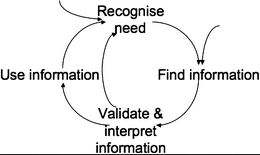
\includegraphics{loop1.png}






% What is trajectory data? 
\subsection{Trajectory Data}


A trajectory is the trace of a moving object - a path through space as a function of time. 
Examples of moving objects could be anything from vehicles to particles - their commonality being that they are entities with positioning or geometrical properties that change over time \cite{Tradef2}. 

The data of trajectories is typically represented by a set of chronologically ordered location points, $ P = \langle x_{n}, y_{n}, t_{n} \rangle $ where $x_{i}, y_{i}$ are geographical coordinates at time $t_{i}$, and \emph{n} is the total number of elements in the series \cite{Tradef1}. When put together, these create a trajectory $ T = \{ P_{1}, P_{2},...,P{n} \} $. 

It is also possible that the data contains information besides the location points themselves. These attributes are either derived from or associated with the data and is often referred to as thematic \cite{Ref1}. Examples of such attributes could be category, the speed of an object at a given time, or what direction the object is facing.  


\subsubsection{Anomaly Detection}

%Using VA to create clusters of trajectories 
\subsubsection{Clustering Trajectories}
%use k-means? http://bl.ocks.org/feyderm/75c18a9143aac50a24e392762f10d6a4
%https://bl.ocks.org/wolfDynamics/8682a6ff548e820d4acb5cd0e87ca603
% //www.npmjs.com/package/density-clustering <- packages in js already available for all of the different kinds of clustering. 

% Why clustering? 
Clustering algorithms can be classified into three
categories: partitioning methods, hierarchical methods and density-based methods.



% What will we conduct research on, how has it been altered (petter har fixat datapunkterna!) 
\subsection{The Dataset}

The chosen dataset for this thesis has its origins from the UCY Computer Graphics Lab \cite{Cyprus}. It consists of a series of splines describing the movement of students walking at a campus area, captured in a video. 

%It could be interesting to render the not so fixed dataset as well. 



    




\subsection{Tools}

HTML is an abbreviation for HyperText Markup Language. It consists of elements representing layout and formatting.  

\subsubsection{DOM}
\subsubsection{D3 - Data Driven Documents}
D3 is a library dedicated to data visualization,  

\subsubsection{JSON}
\subsubsection{Browser Architecture}

Browsers consist of several modular pieces, each responsible for certain functionalities:
\begin{itemize}
    \item UI layer - draws the user interface, e.g. windows and buttons. 
    \item Rendering engine - parses, tokenizes and renders the HTML. 
    \item Network layer - manages network operations needed to retrieve HTML and assets.
    \item JavaScript engine - interprets and executes the JavaScript code. 
\end{itemize}


\subsection{Related Work}
 \begin{itemize}
     \item Visual Analytics Tools for Analysis of Movement Data
     \item An Exploratory Spatial Data Analysis (ESDA) Toolkit for the Analysis of Activity/Travel Data
 \end{itemize}

\section{Method}

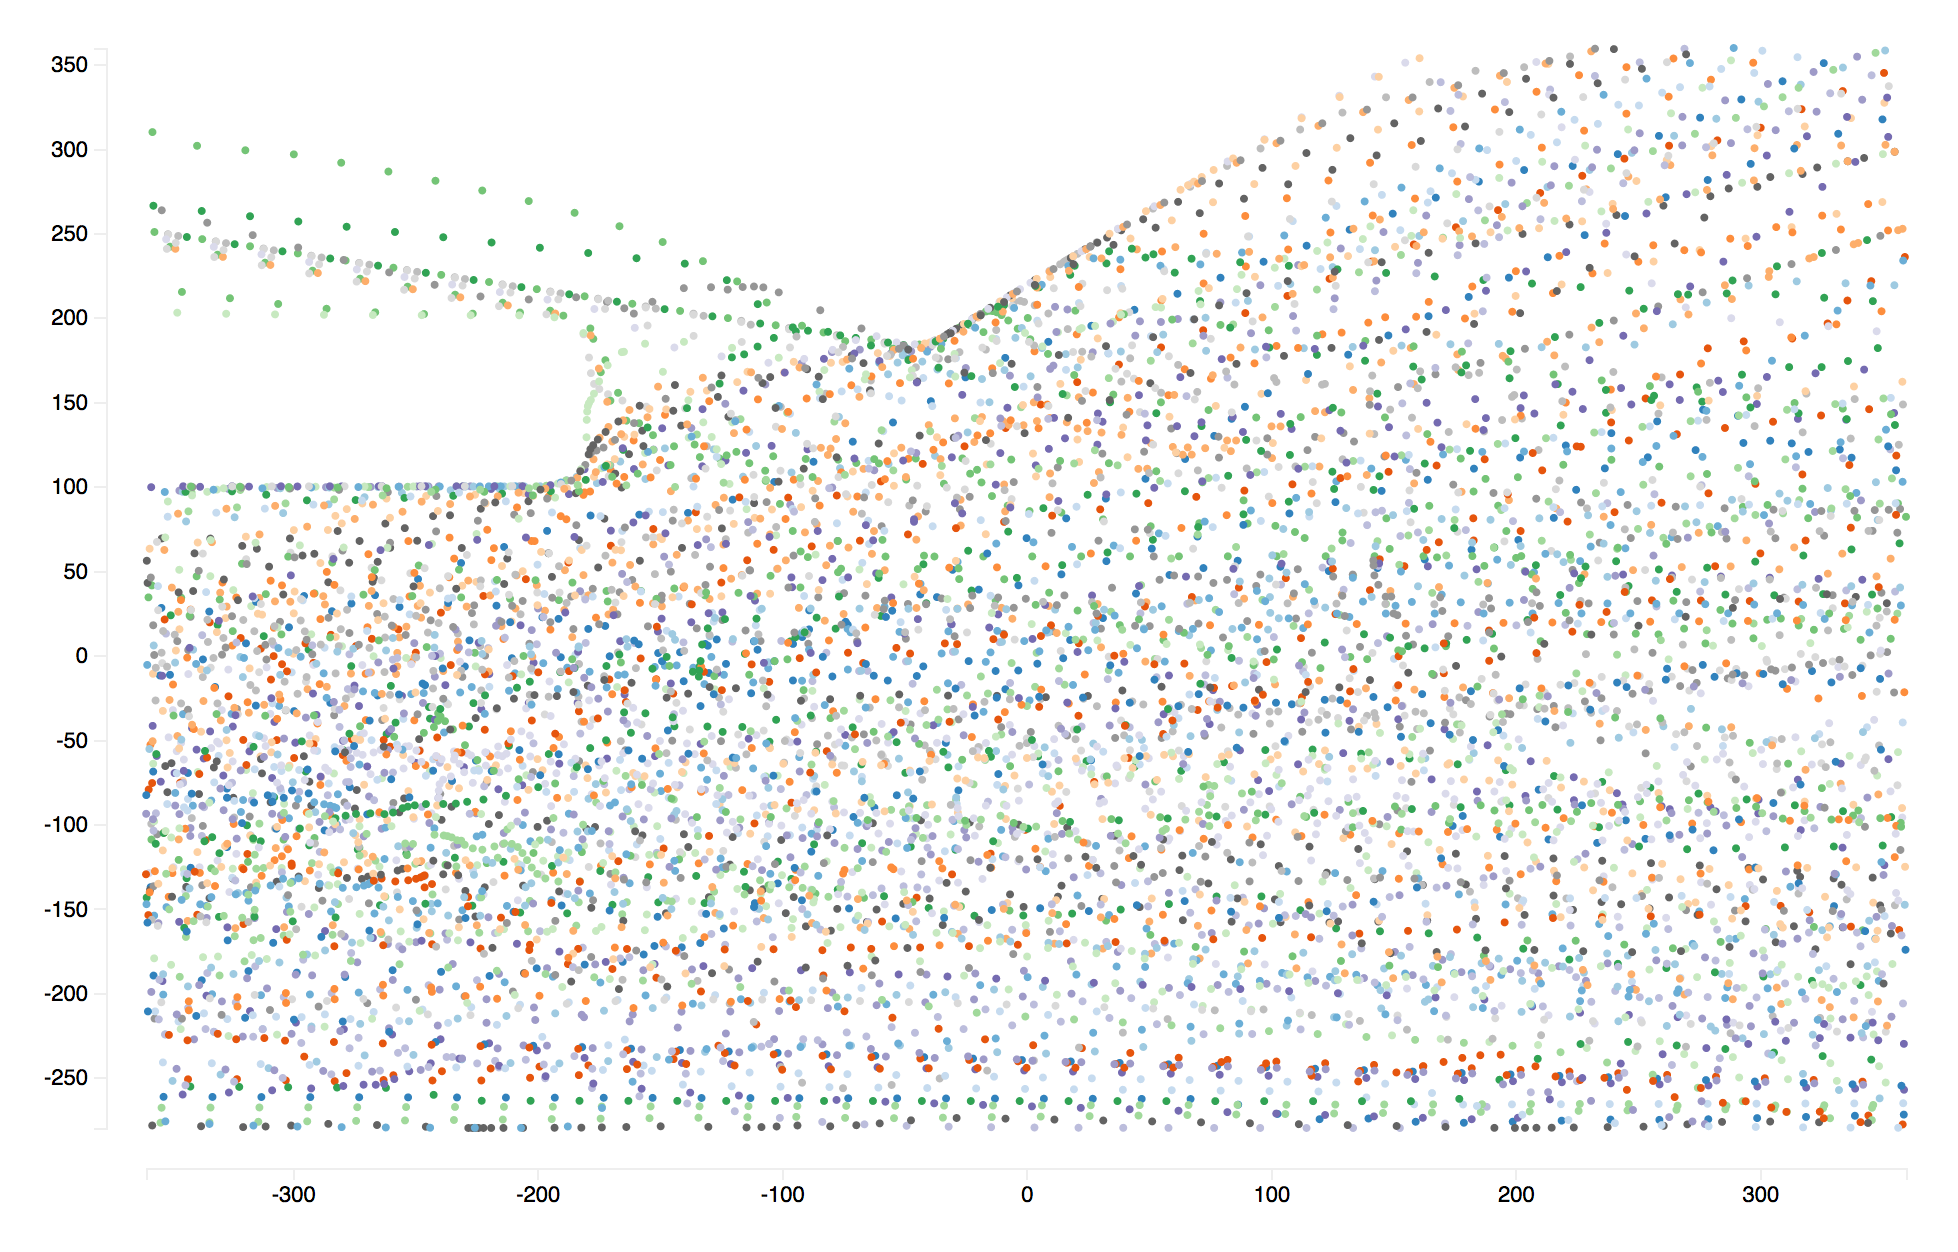
\includegraphics[height= 7cm, width=14cm]{scatterplot.png}




\section{Results and analysis}

\section{Discussion}

\section{Conclusion}

\printbibliography

\end{document}
